\chapter{Das BNN}
Bei unserem Neuronalen Netz handelt es sich um ein binäres Netzwerk. Im Folgenden werden die Anpassungen, beziehungsweise die verwendeten Komponenten beschrieben.
\section{Aktivierungsfunktion}
In neuronalen Netzwerken kann, wie in Kapitel \ref{sec:activation} beschrieben, eine ganze Reihe von Aktivierungsfunktionen verwendet werden. Jede dieser Funktionen hat, je nach Anwendungskontext, verschiedene Vor- und Nacheile.\\
Für BNNs ist hier die $sign(x)$ Funktion eine populäre Wahl.
\begin{figure}[h]
	\centering
		\begin{tikzpicture}[]
	\begin{axis}[
	axis lines=middle,
	xlabel=$x$,
	ylabel={$sign(x)$},
	xmin=-3, xmax=3,
	ymin=-1.5, ymax=1.5,
	ytick={0, 1},
	extra y ticks={-1},
	extra y tick style={
		tick label style={anchor=west, xshift=3pt},
	},
	function line/.style={
		red,
		thick,
		samples=2,
	},
	single dot/.style={
		red,
		mark=*,
	},
	empty point/.style={
		only marks,
		mark=*,
		mark options={fill=white, draw=black},
	}
	]
	\addplot[function line, domain=\pgfkeysvalueof{/pgfplots/xmin}:0] {-1};
	\addplot[function line, domain=0:\pgfkeysvalueof{/pgfplots/xmax}] {1};
	\addplot[single dot] coordinates {(0, 0)};
	\addplot[empty point] coordinates {(0, -1) (0, 1)};
	\end{axis}
	\end{tikzpicture}
	\caption{Die Vorzeichenfunktion}
	\label{fig:sign}
\end{figure} 
Diese überführt die Aktivierungen direkt in binäre Werte. Da für die \textit{backpropagation} allerdings die Ableitung der Aktivierungsfunktion benötigt wird und die Vorzeichenfunktion nicht stetig differenzierbar ist, wird diese approximiert. In unserem Netzwerk wird sie, wie häufig verwendet, durch die \textit{hard tanH} Funktion approximiert \cite{DBLP:journals/corr/abs-2012-00938}. Diese ist, in den Ableitungen, günstiger zu berechnen als die Funktion \textit{sign} und ist bei Werten $x\leq-1 \vee x \geq 1$ gleich zur Vorzeichenfunktion.
\section{Binärer Linear-Layer}
Für die Binarisierung der Linear-Layer wurde eine \textit{Wrapper-Klasse} für die Pytorch-Klasse \textit{nn.linear} erstellt.

\begin{figure}[H]
	\centering
	\begin{tikzpicture}[minimum height=0.75cm,minimum width=2cm,line width = 0.25mm]
	\node[rectangle,draw=black] (input) {Eingabe};
	\node[rectangle,draw=black] (weights) at(3,0) {Gewichte};
	\node[rectangle,draw=black] (sign1) at(0,-1.5)  {sign(x)};
	\node[rectangle,draw=black] (sign2) at(3,-1.5)  {sign(x)};
	\node[rectangle,draw=black] (nnlinear) at(1.5,-3)  {nn.linear};
	
	\node[scale=0.01] (weightsin) at(4.5,0) {};
	\node[scale=0.01] (inputin) at(0,1.5) {};
	
	
	\node[draw=black,rectangle, fit= (input) (weights) (sign1) (sign2),inner sep=0.4cm] (bnn)   {};
	\node [yshift=0.4cm,xshift=-1.5cm] (bnnlabel) at (bnn.north east) {BinarizedLinear};
	
	
	
	\draw [->,dotted,line width = 0.4mm] (weightsin) -- (weights);
	\draw [->,line width = 0.4mm] (inputin) -- (input);
	
	\draw [->,line width = 0.4mm] (input) -- (sign1) ;
	\draw [->,line width = 0.4mm] (weights) -- (sign2);
	
	\draw [->,line width = 0.4mm] (sign1) -- (nnlinear) ;
	\draw [->,line width = 0.4mm] (sign2) -- (nnlinear);
	
	
	\end{tikzpicture}
	\caption{Aufbau des binären Linear-layer}
	\label{fig:bln}
\end{figure}
Wie in Abbildung \ref{fig:bln} zu erkennen, erhält der binäre Linear-Layer, wie normaler Weise \textit{nn.linear}, die Ausgaben der vorherigen Schicht. Diese werden im Folgenden über die Vorzeichenfunktion binarisiert.\\
Die Gewichte, welche über das Training aktualisiert werden, werden bei erster Verwendung ebenfalls binarisiert. Im folgenden übernimmt die Pytorch-Klasse \textit{nn.linear} die Berechnung der Aktivierung der Neuronen. Da die Berechnung der Aktivierungen also immer auf binären Gewichten und Eingaben geschieht, ist das Training binär.

\section{BatchNorm}
Die Rolle des \textit{BatchNorm-Layers} in nicht-binären Neuronalen-Netzwerken ist eine leicht andere als in unserem BNN. Durch \textit{BatchNorm} werden die Eingaben einer Schicht, innerhalb eines \textit{Batches}, normalisiert. Hier wird dafür gesorgt, dass \textit{Batches} einen Mittelwert von Null und eine Standartabweichung von Eins haben\cite{batchnorm} .\\ 
Durch diese reduzierte Streuung der Werte, können in Neuronalen Netzen höhere Lernraten verwendet werden, da stark ausschlagende Daten nicht zu einer starken Überanpassung führen.\\
Bei binären Netzwerken hat dies, aufgrund der diskreten Kantengewichte,einen weniger großen Effekt.In BNNs erfüllt die \textit{BatchNorm} Schicht eine zentrale Rolle für das Lernen des Netzwerkes. Primär dient die Normalisierung der Schicht dazu, das \textit{expolding-gradient} Problem zu verhindern. Hier wird beim Training des Netzwerkes, welches die Error-Werte reduzieren soll, ein sehr hoher Error-Wert akkumuliert. Dies führt zu einer zu starken Anpassung der Gewichte, welche folgend zu einer niedrigeren Genauigkeit führt\cite{DBLP:journals/corr/abs-1909-09139}.\\
 Da durch Auftreten des \textit{exploding gradients} die Genauigkeit stark abgesenkt wird, kann dieses Netzwerk sich, ab einer gewissen Schwelle, nicht mehr verbessern. Der stetige Lernerfolg wird hier durch regelmäßige Überkorrekturen nichtig gemacht.
\begin{figure}[H]
	\centering
	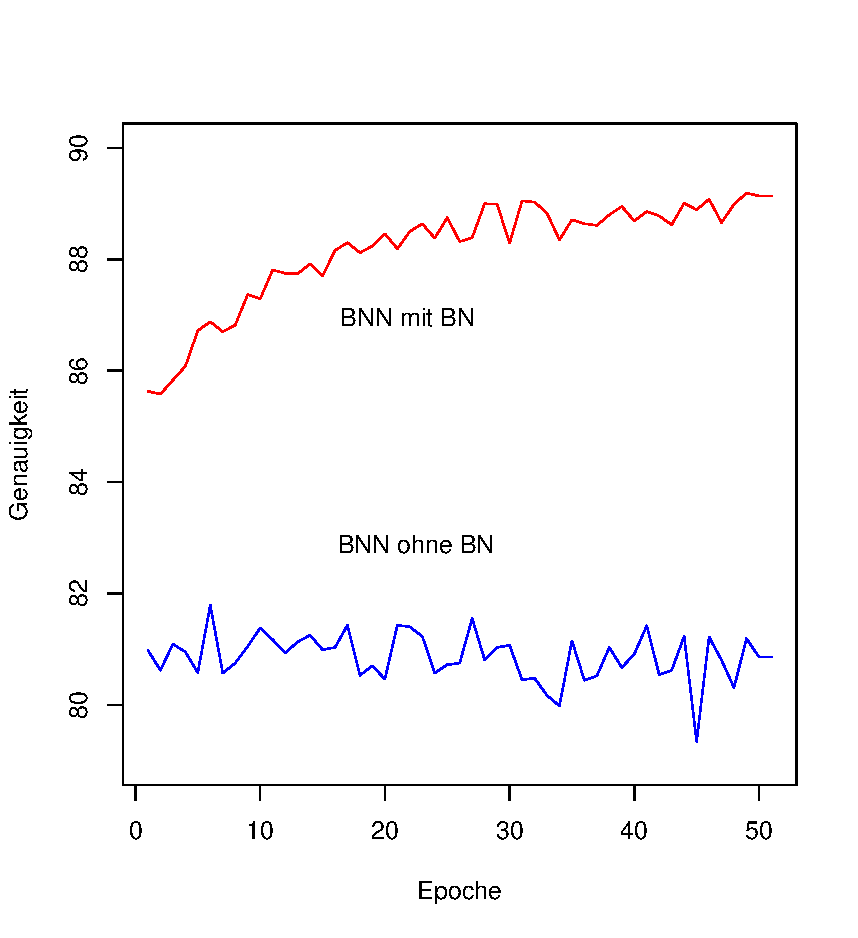
\includegraphics[scale=0.7]{./bilder/_plot_batchnorm}
	\caption{Training mit und ohne BatchNorm}
	\label{fig:bn}
\end{figure}
Der Versuch in Abbildung \ref{fig:bn} zeigt einen Vergleich des Netzwerkes mit und ohne \textit{BatchNorm}. Hierfür wurde ein Netzwerk für 50 Epochen trainiert. Nach jeder Epoche wurde die Genauigkeit getestet. Anschließend wird das Training fortgesetzt. Um eine bessere Vergleichbarkeit zu erzielen, wurden die Bilder über die Schwellwert-Methode binarisiert.\\

Wie in Abbildung \ref{fig:bn} zu sehen ist, performt das Netzwerk mit \textit{BatchNorm} Schicht zu jeder Trainingsdauer besser als ohne \textit{BatchNorm} Schicht. Während in den ersten 20 Epochen mit \textit{BatchNorm} ein klarer Aufwärtstrend zu erkennen ist, stagniert die Genauigkeit ohne \textit{BatchNorm} zwischen 79\% und 82\%. Hier sind besonders gut die starken Einbrüche nach Unten zu erkennen, die mit \textit{BN} deutlich abgeschwächt sind. Diese zeigen besonders deutlich den starken Genauigkeitsverlust, der durch \textit{exploding gradients} verursacht wird. Die Konsequenz ist, dass eine längere Trainingsdauer keine Verbesserung des Netzwerkes mehr bedeutet, was bedeutet, dass die Konvergenz-Schwelle bei $< 82$ erreicht ist. Ab dieser Schwelle verbessert sich das Netzwerk ohne \textit{BN} nicht mehr.


\section{Auswertung der letzten Schicht}
Um am Ende das Ergebnis des Netzwerkes auszuwerten, müssen die Ergebnisse des letzten \textit{Linear-Layers} normalisiert werden. Diese Normalisierung entscheidet, ob ein Neuron feuert oder nicht. Für die Normalisierung der Daten wird hier die \textit{logsoftmax(x)} Funktion verwendet. Durch \textit{softmax(x)} werden die Aktivierungen der letzten Schicht so normalisiert, dass ihre Summe Eins ergibt. Dies ist mit Wahrscheinlichkeiten zu vergleichen, mit der das Bild die jeweilig zugeordnete Zahl widerspiegelt. Um bessere Ergebnisse in Kombination mit der Verlustfunktion, \textit{negative log likelihood loss}, zu erzielen, wird die \textit{logsoftmax}-Funktion verwendet.\\
Da bei der Anwendung des MNIST-Datensatzes immer nur das Neuron ausgewählt werden sollte, da immer nur eine Zahl auf einem Bild abgebildet ist, wird bei der Auswertung über die \textit{argmax}-Funktion das aktivste Neuron ausgewählt. Dieses entspricht dann der Zahl, die am wahrscheinlichsten abgebildet ist.


\section{Verluste durch binäre Linear-Layer}
Durch die binarisierung der \textit{Linear-Layer} ist zu vermuten, dass diese, im Vergleich zu normalen \textit{Linear-Layer}, etwas schlechter performen. Dies ist der Fall, da die Anzahl der möglichen Kantengewichte stark, auf Null und Eins, eingeschränkt ist. 
\begin{figure}[h]
	\centering
	\begin{tabular}{|c|c|c|}\hline
		Durchgang&binarär&normal\\\hline
		1&88.29&97.43\\\hline
		2&87.32&96.98\\\hline
		3&87.19&97.2\\\hline
	\end{tabular}
\caption{Verlustmessung für den \textit{Linear-Layer}}
\label{fig:linar-layer-verluste}
\end{figure}


Trainiert wurde hier das gleiche Netzwerk, ein mal mit binären \textit{Linear-Layern}, das andere mal mit normalen \textit{Linear-Layer}. Jedes Netzwerk wurde für 50 Epochen trainiert, bevor die Genauigkeit ausgewertet wurde. Um sicher zu gehen, ob die Genauigkeit gegen diesen Wert konvergiert, wurde jede Messung drei mal wiederholt.\\
Wie in Abbildung \ref{fig:linar-layer-verluste} zu sehen, leidet die Genauigkeit des Netzwerkes beachtlich unter der Binarisierung der \textit{Linear-Layer}. Der Mittelwert für das Training mit normalem \textit{Linear-Layer} ist hierbei $97,2\%$, während bei binären Schichten ein Durchschnitt von $87,6\%$ erreicht wird. Es ist klar zu sehen, dass die Einschränkung der Gewichte auf Null und Eins und der damit einhergehende Granularitätsverlust, sich stark auf die Genauigkeit des Netzwerkes, bei gleicher Größe, auswirken. 

